\documentclass[11pt]{article}
% Shared preamble of the RMC kernel write-ups (% Shared preamble of the RMC kernel write-ups (% Shared preamble of the RMC kernel write-ups (\input{preamble} after \documentclass).
\usepackage[margin=1in]{geometry}
\usepackage{amsmath,amssymb,bm}
\usepackage{graphicx}
\usepackage{booktabs}
\usepackage{hyperref}

\newcommand{\dd}{\,\mathrm{d}}
\newcommand{\Ein}{E}
\newcommand{\Eout}{E'}
\newcommand{\Ecm}{E_{c}}
\newcommand{\mucm}{\mu_{c}}
\newcommand{\mulab}{\mu_0}

% Common closing section: how the verification figures are produced
\newcommand{\verificationmethod}{%
Each figure is produced by \texttt{verification/verify\_laws.py}. For an incident
energy $\Ein$ along $+z$, $10^6$ collisions are sampled with MC/DC's own reaction
sampler (\texttt{sample\_elastic\_scattering}, \texttt{sample\_inelastic\_scattering}
or \texttt{sample\_fission}), and every emitted neutron is histogrammed in
$48 \times 24$ bins of $(\Eout, \mulab)$, with $\mulab$ the lab cosine to $+z$. The
inverted kernel used by RMC is integrated over the same bins (Gauss--Legendre panels;
two-body lines are split where $\mulab^*(\Eout)$ crosses a cosine edge), multiplied by
the number of collisions, and compared with a $\chi^2$ test over bins with at least 5
expected counts (the rest pooled into one bin). The tables list $\chi^2/\mathrm{dof}$,
its $p$-value, the emitted neutrons per collision (sampled vs.\ the integral of the
inverted kernel), and the largest relative change of a bin integral when the
quadrature panels are doubled. Left panels: outgoing-energy marginal; middle:
lab-cosine marginal; right: per-bin $z = (\text{sampled} - \text{inverted}) /
\sqrt{\text{inverted}}$.}
 after \documentclass).
\usepackage[margin=1in]{geometry}
\usepackage{amsmath,amssymb,bm}
\usepackage{graphicx}
\usepackage{booktabs}
\usepackage{hyperref}

\newcommand{\dd}{\,\mathrm{d}}
\newcommand{\Ein}{E}
\newcommand{\Eout}{E'}
\newcommand{\Ecm}{E_{c}}
\newcommand{\mucm}{\mu_{c}}
\newcommand{\mulab}{\mu_0}

% Common closing section: how the verification figures are produced
\newcommand{\verificationmethod}{%
Each figure is produced by \texttt{verification/verify\_laws.py}. For an incident
energy $\Ein$ along $+z$, $10^6$ collisions are sampled with MC/DC's own reaction
sampler (\texttt{sample\_elastic\_scattering}, \texttt{sample\_inelastic\_scattering}
or \texttt{sample\_fission}), and every emitted neutron is histogrammed in
$48 \times 24$ bins of $(\Eout, \mulab)$, with $\mulab$ the lab cosine to $+z$. The
inverted kernel used by RMC is integrated over the same bins (Gauss--Legendre panels;
two-body lines are split where $\mulab^*(\Eout)$ crosses a cosine edge), multiplied by
the number of collisions, and compared with a $\chi^2$ test over bins with at least 5
expected counts (the rest pooled into one bin). The tables list $\chi^2/\mathrm{dof}$,
its $p$-value, the emitted neutrons per collision (sampled vs.\ the integral of the
inverted kernel), and the largest relative change of a bin integral when the
quadrature panels are doubled. Left panels: outgoing-energy marginal; middle:
lab-cosine marginal; right: per-bin $z = (\text{sampled} - \text{inverted}) /
\sqrt{\text{inverted}}$.}
 after \documentclass).
\usepackage[margin=1in]{geometry}
\usepackage{amsmath,amssymb,bm}
\usepackage{graphicx}
\usepackage{booktabs}
\usepackage{hyperref}

\newcommand{\dd}{\,\mathrm{d}}
\newcommand{\Ein}{E}
\newcommand{\Eout}{E'}
\newcommand{\Ecm}{E_{c}}
\newcommand{\mucm}{\mu_{c}}
\newcommand{\mulab}{\mu_0}

% Common closing section: how the verification figures are produced
\newcommand{\verificationmethod}{%
Each figure is produced by \texttt{verification/verify\_laws.py}. For an incident
energy $\Ein$ along $+z$, $10^6$ collisions are sampled with MC/DC's own reaction
sampler (\texttt{sample\_elastic\_scattering}, \texttt{sample\_inelastic\_scattering}
or \texttt{sample\_fission}), and every emitted neutron is histogrammed in
$48 \times 24$ bins of $(\Eout, \mulab)$, with $\mulab$ the lab cosine to $+z$. The
inverted kernel used by RMC is integrated over the same bins (Gauss--Legendre panels;
two-body lines are split where $\mulab^*(\Eout)$ crosses a cosine edge), multiplied by
the number of collisions, and compared with a $\chi^2$ test over bins with at least 5
expected counts (the rest pooled into one bin). The tables list $\chi^2/\mathrm{dof}$,
its $p$-value, the emitted neutrons per collision (sampled vs.\ the integral of the
inverted kernel), and the largest relative change of a bin integral when the
quadrature panels are doubled. Left panels: outgoing-energy marginal; middle:
lab-cosine marginal; right: per-bin $z = (\text{sampled} - \text{inverted}) /
\sqrt{\text{inverted}}$.}


\title{Inverted kernel: discrete-level inelastic scattering (ACE Law 3)}
\date{}

\begin{document}
\maketitle

\noindent Code: \texttt{delta\_lab\_line} (level branch) in
\texttt{mcdc/rmc/reaction.py}, \texttt{level\_*} in \texttt{mcdc/rmc/kinematics.py},
\texttt{\_delta\_inner} in \texttt{mcdc/rmc/kernel.py}.

\section{What MC/DC samples}

\noindent Source: \acespec{4.3.11.3} (level-scattering parameters).
The frame and angular interpolation below describe the MC/DC sampler; the
COM-to-lab transformation is derived in \texttt{frames\_and\_azimuth.tex}.

\texttt{sample\_inelastic\_scattering} with a level-scattering spectrum in the COM
frame: the COM outgoing energy is fixed,
\begin{equation}
  \Ecm = C_2\,(\Ein - C_1),\qquad C_1 = \frac{A+1}{A}|Q|,\quad C_2 = \left(\frac{A}{A+1}\right)^2 ,
\end{equation}
$\mucm$ is isotropic or drawn from the reaction's angular multi-table (unscaled,
table $i$ or $i+1$ with probabilities $1-f$, $f$ as for elastic scattering), and the
classical COM-to-lab relations of \texttt{frames\_and\_azimuth.tex} give
$(\Eout, \mulab)$. Below threshold, $\Ecm \le 0$ and nothing is emitted. The yield $Y$
is the reaction multiplicity (or a tabulated yield, see
\texttt{multi\_spectrum\_yield.tex}).

\section{Inverted kernel}

For fixed $\Ecm$, $\Eout = \Ecm + s^2 + 2\mucm s\sqrt{\Ecm}$ with $s = \sqrt{\Ein}/(A+1)$
is affine in $\mucm$, so
\begin{equation}
  \mucm^*(\Eout) = \frac{(A+1)^2(\Eout - \Ecm) - \Ein}{2(A+1)\sqrt{\Ein\Ecm}},\qquad
  \left|\frac{\dd\mucm}{\dd\Eout}\right| = \frac{A+1}{2\sqrt{\Ein\Ecm}},
\end{equation}
\begin{equation}
  \mulab^*(\Eout) = \mucm^*\sqrt{\frac{\Ecm}{\Eout}} + \frac{1}{A+1}\sqrt{\frac{\Ein}{\Eout}},
\end{equation}
and the lab kernel is the line
\begin{equation}
  f_L(\Eout, \mulab \mid \Ein) = Y\,p_c(\mucm^*; \Ein)\,\frac{A+1}{2\sqrt{\Ein\Ecm}}\;
  \delta\big(\mulab - \mulab^*(\Eout)\big),
\end{equation}
on the support $\Eout \in [(\sqrt{\Ecm} - s)^2, (\sqrt{\Ecm} + s)^2]$ ($\mucm = \mp1$).
In the transfer moments the $\Eout$ integral over an outgoing bin becomes a closed-form
$\mucm$ interval, so only bins inside the support are visited.

\section{Verification}
\verificationmethod

\begin{center}
\begin{tabular}{rrrrrrr}
\toprule
$E$ [eV] & samples & bins & $\chi^2/\mathrm{dof}$ & $p$ & yield (sampled / inverted) & quad. err. \\
\midrule
8e+06 & 1e+06 & 71 & 74.6/71 & 0.363 & 1.00000 / 1.00000 & 6.7e-09 \\
1.4e+07 & 1e+06 & 71 & 67.1/71 & 0.608 & 1.00000 / 1.00000 & 8.1e-08 \\
\bottomrule
\end{tabular}

\end{center}

\begin{figure}[h]
  \centering
  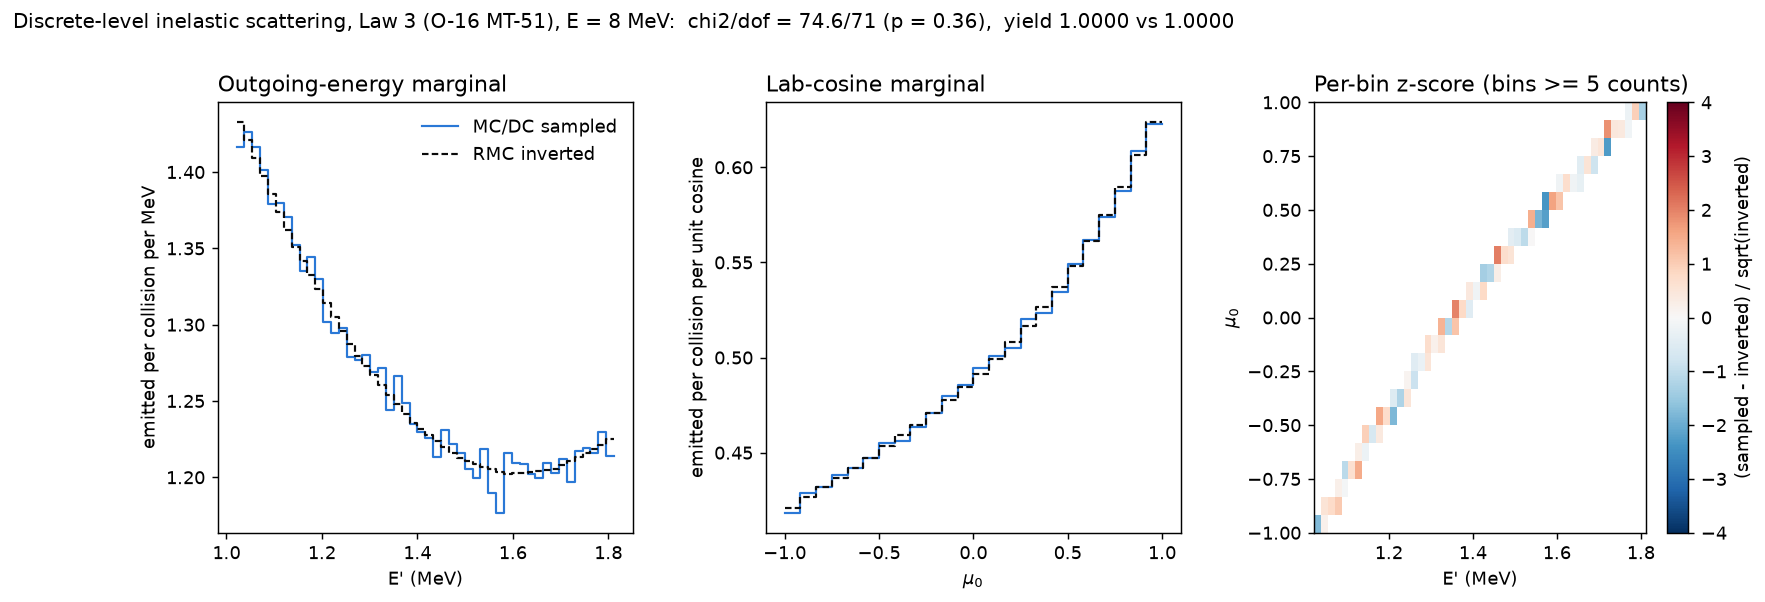
\includegraphics[width=\textwidth]{figures/level/level_E8e06.png}
  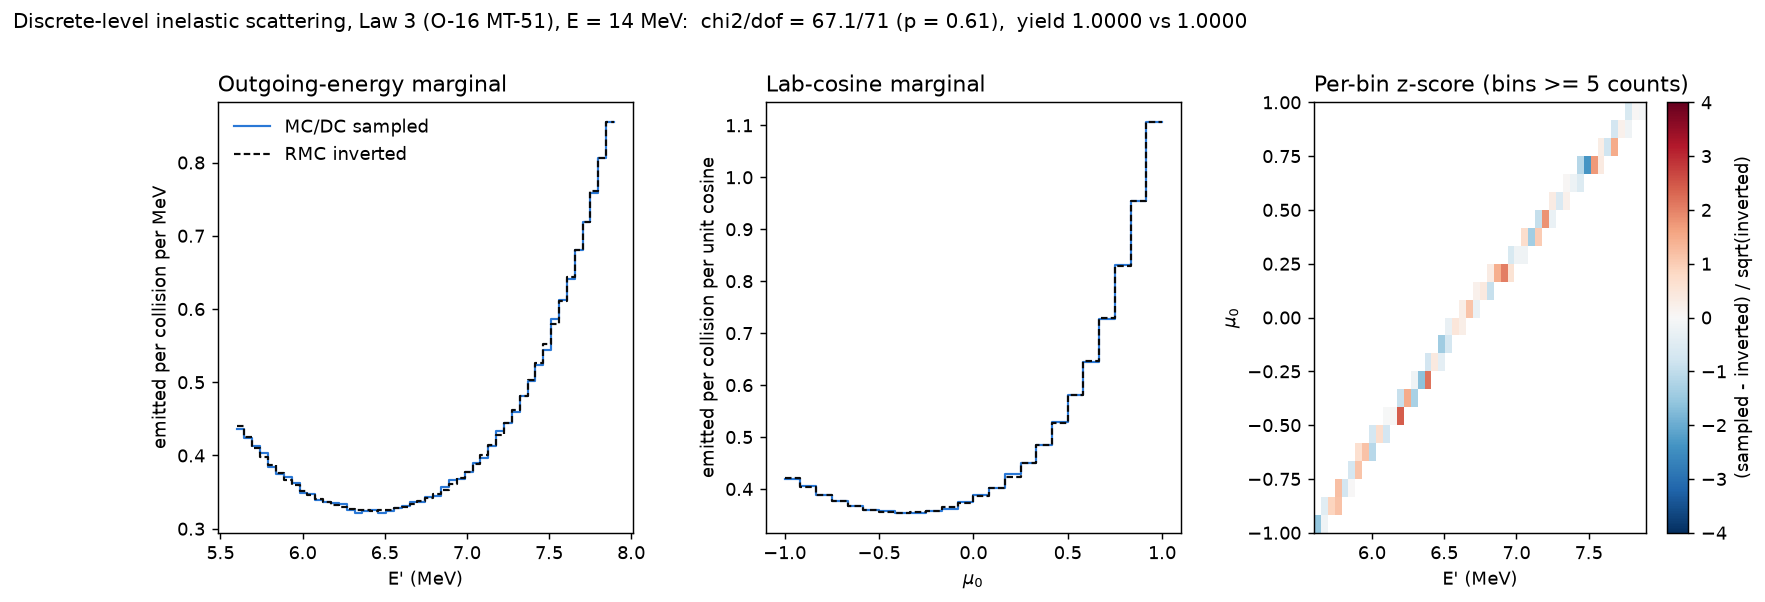
\includegraphics[width=\textwidth]{figures/level/level_E1p4e07.png}
  \caption{O-16 MT-51 (first excited level, tabulated COM angular data) at 8 and
  14\,MeV.}
\end{figure}

\end{document}
